\item Borrar toda la información del cliente \textbf{Paul Stevenson}.

\begin{lstlisting}
orders = orders − π orderid, orderdate, shipdate, shipmode, customerid, productid, quantity
         (σ customername = 'Paul Stevenson' (customer ⨝= orders))

customer = customer − σ customername = 'Paul Stevenson' (customer)
\end{lstlisting}

Paul Stevenson (PS-18970) tiene 6 renglones de orden en 5 órdenes.
Se eliminan primero sus órdenes y después su registro en \texttt{customer}
para respetar la llave foránea. En Relax, la verificación se hace con
\texttt{orders\_sin\_paul} y \texttt{customer\_sin\_paul}; el join externo
derecho se escribe \texttt{right join}.

% ==========================================
% Página de mayor tamaño para los árboles y las tuplas
% (misma técnica que la Práctica 05)
% ==========================================
\clearpage
\pdfpagewidth=35cm
\pdfpageheight=32cm
\setlength{\textwidth}{34cm}
\setlength{\hsize}{34cm}
\setlength{\oddsidemargin}{\dimexpr(\pdfpagewidth-\textwidth)/2 - 1in\relax}
\setlength{\evensidemargin}{\oddsidemargin}
\setlength{\textheight}{31cm}
\setlength{\vsize}{31cm}
\setlength{\headheight}{0pt}
\setlength{\headsep}{0pt}
\setlength{\topmargin}{\dimexpr(\pdfpageheight-\textheight)/2 - 1in\relax}
\thispagestyle{empty}
\vspace*{0.2cm}
\centering
\begin{tabular}{@{}c@{\hspace{0.5cm}}c@{}}
\begin{minipage}[t]{0.42\textwidth}
  \centering
  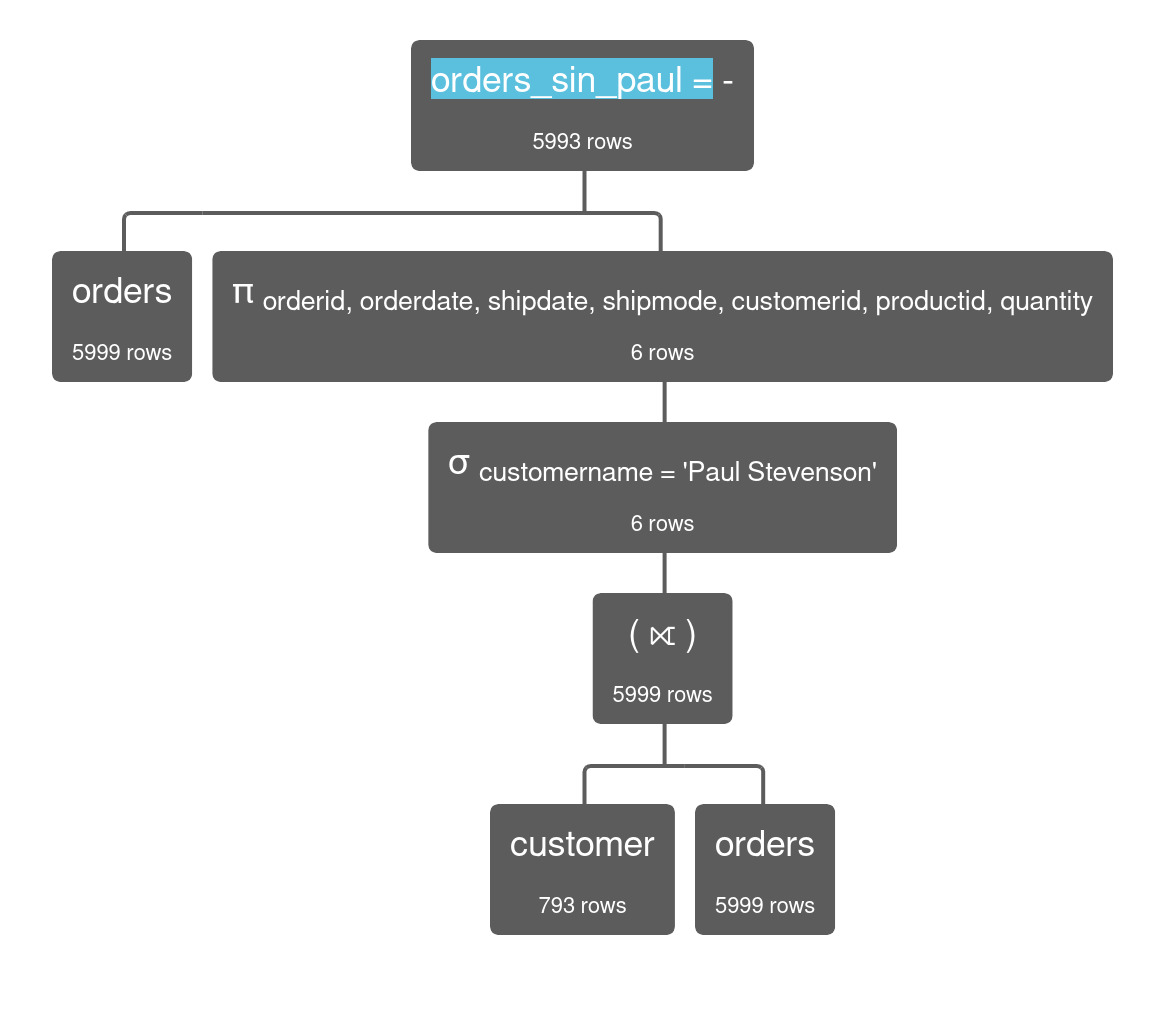
\includegraphics[width=\linewidth]{figuras/3a_arbol.jpg}\\[0.1cm]
  {\small Árbol de \texttt{orders\_sin\_paul}}
\end{minipage} &
\begin{minipage}[t]{0.42\textwidth}
  \centering
  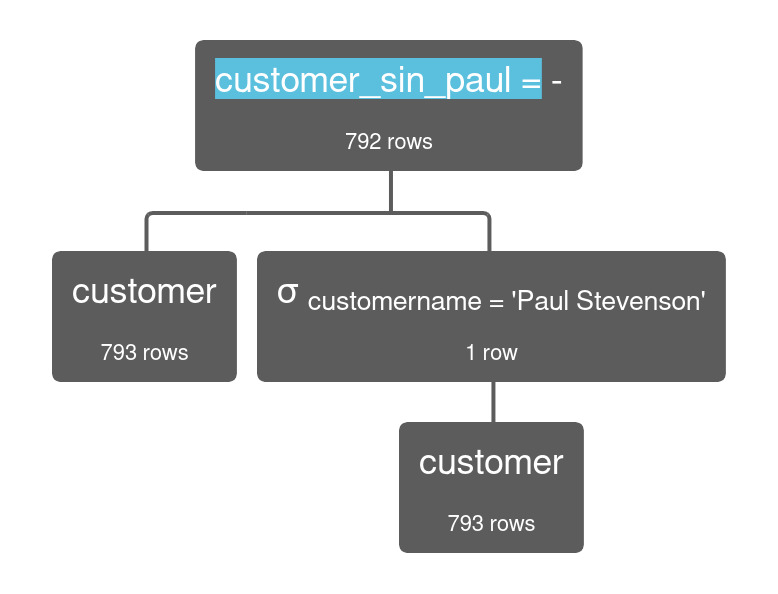
\includegraphics[width=\linewidth]{figuras/3a_arbol_customer.jpg}\\[0.1cm]
  {\small Árbol de \texttt{customer\_sin\_paul}}
\end{minipage}
\end{tabular}

\vspace{0.35cm}
\begin{tabular}{@{}c@{\hspace{0.5cm}}c@{}}
\begin{minipage}[t]{0.42\textwidth}
  \centering
  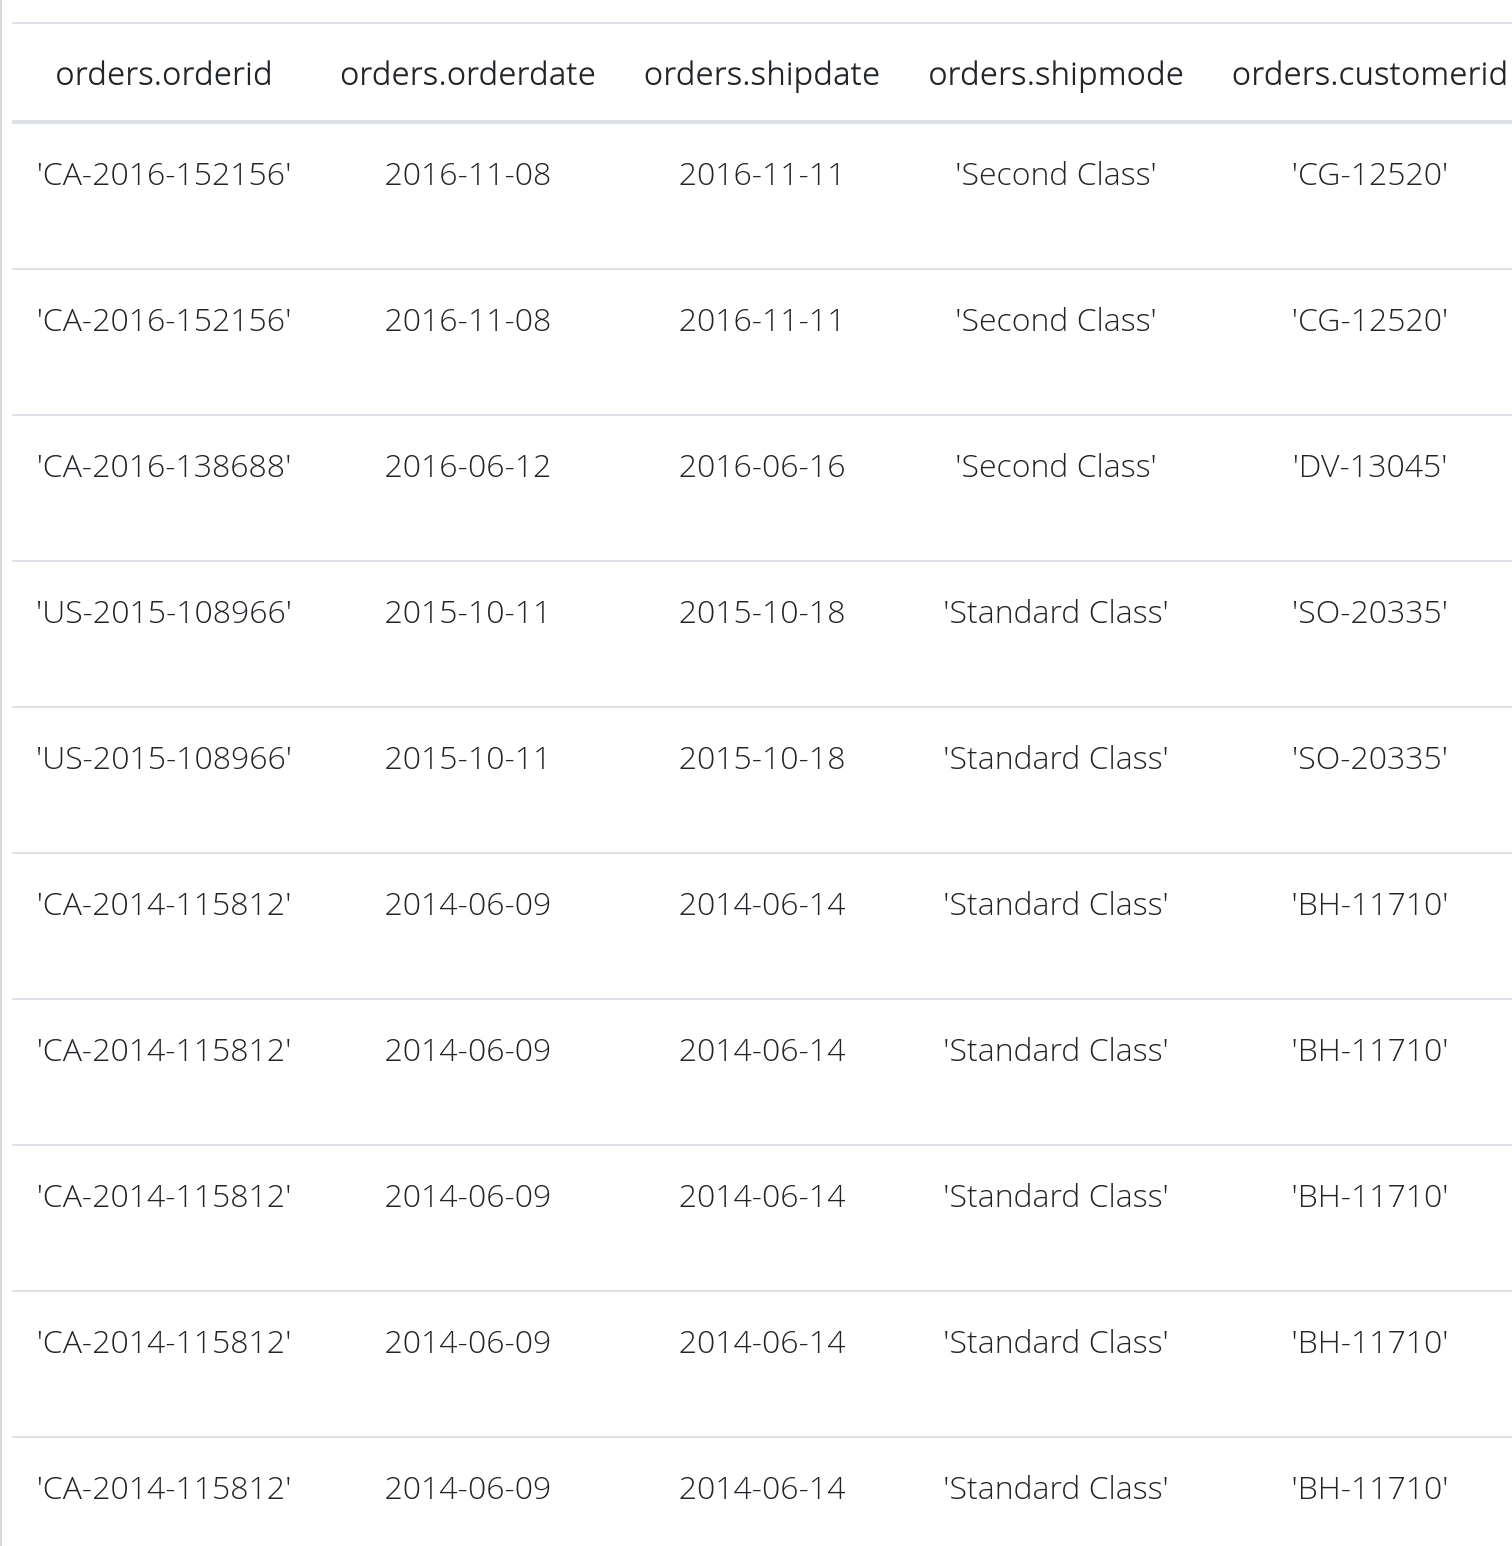
\includegraphics[width=\linewidth]{figuras/3a_tuplas.png}\\[0.1cm]
  {\small Primeros renglones de \texttt{orders\_sin\_paul}}
\end{minipage} &
\begin{minipage}[t]{0.42\textwidth}
  \centering
  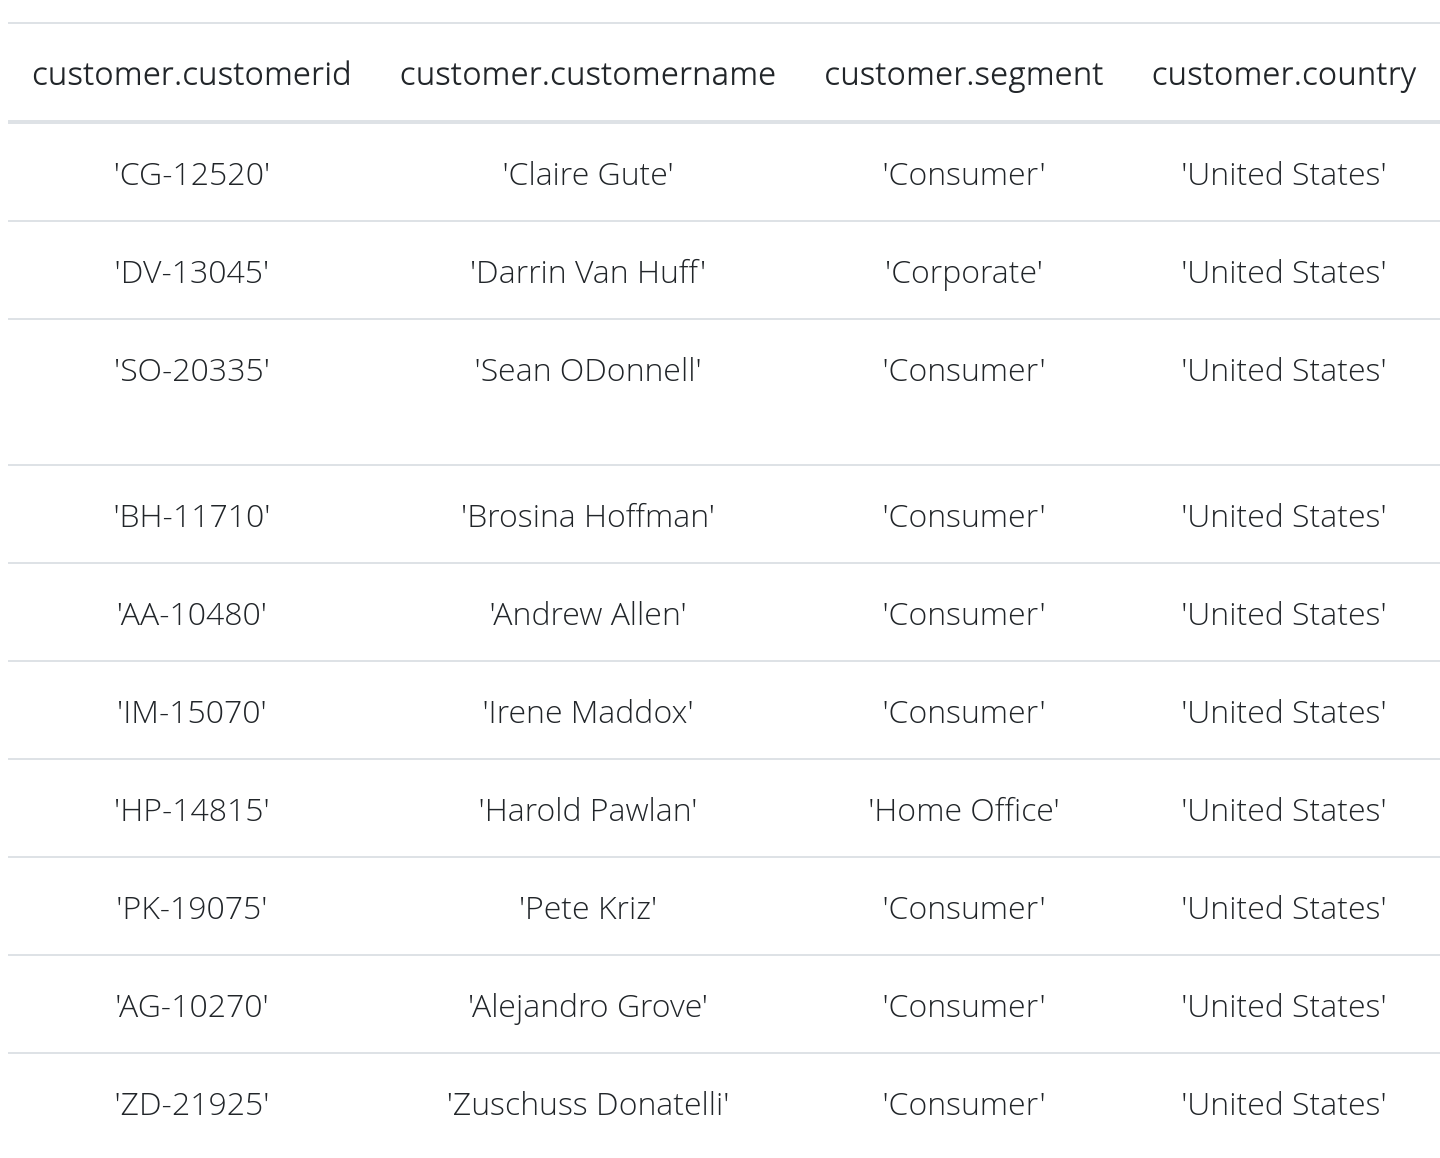
\includegraphics[width=\linewidth]{figuras/3a_tuplas_customer.png}\\[0.1cm]
  {\small Primeros renglones de \texttt{customer\_sin\_paul}}
\end{minipage}
\end{tabular}

\vspace{0.3cm}
{\small Las tuplas mostradas son los primeros renglones de las relaciones
resultantes; Paul Stevenson ya no aparece en \texttt{orders\_sin\_paul}
ni en \texttt{customer\_sin\_paul}.}
\clearpage
\restoregeometry
\pdfpagewidth=\paperwidth
\pdfpageheight=\paperheight
